\documentclass[12pt]{article}

% Set page size and margins
% Replace `letterpaper' with `a4paper' for UK/EU standard size
\usepackage[a4paper,top=2cm,bottom=2cm,left=2cm,right=2cm,marginparwidth=1.75cm]{geometry}

% Language and encoding
\newcommand{\dumblang}[2]{{#2}}
%\usepackage{\dumblang{polski}{english}}
%\usepackage{[\dumblang{polish}{english}]{babel}}
\usepackage[ \dumblang{polish}{english} ]{babel}
\usepackage[utf8]{inputenc}

% Formatting
\usepackage{float}
\usepackage{graphicx}
\usepackage{anyfontsize}

% Math
\usepackage{amsmath}
\usepackage{mathtools}
\usepackage{extpfeil}


% Table of contents
\usepackage{blindtext}
\usepackage{titlesec}

% Other Stuff
\usepackage[colorlinks=true, allcolors=blue]{hyperref}
\usepackage{comment}
\usepackage{multicol}
\usepackage{listings}
\usepackage[export]{adjustbox}[2011/08/13]

% Add manual tabulator 
\usepackage{tabto}

%
%\usepackage[draft,nosingleletter]{impnattypo}

% Plot
\usepackage{pgfplots}
\usepackage{pgfplotstable}

% Rysunki rysuneczki:
\usepackage[european, american currents, americanvoltages, RPvoltages, cute inductor]{circuitikz} % rysowanie schematów <- super dokumentacje
\usepackage{tikz} % <- rysunki ogólne ale dokumentacja do dupy
\usepackage{pdfpages}

% \usepackage[utf8]{inputenc}
\usepackage{newunicodechar}
\newunicodechar{²}{\ensuremath{{}^2}}


\hypersetup{
  colorlinks = true,
  linkcolor  = black
}

\titleformat{\section}
{\Large \bfseries}
{\thesection.}
{0.5em}
{}[\titlerule]

\titleformat{\subsection}
{\large \bfseries}
{\thesubsection.}
{0.5em}
{}[]

\newtheorem{thm}{Twierdzenie}
\DeclareMathOperator\sinc{sinc}
\DeclareMathOperator\sgn{sgn}
\DeclareMathOperator{\kron}{d}



\newcommand{\xrlh}{\xrightleftharpoons}
\newcommand{\FT}{\xrightleftharpoons[ICFT]{CFT} }
\newcommand{\unit}{\operatorname{u}}
\newcommand{\LT}{\xrightleftharpoons[\mathcal{L}^{-1}]{\mathcal{L}}}
\newcommand{\ZZ}{\mathcal{Z}}

% Włącz numerację w sposób NumerSekcji.NumerRównania
\numberwithin{equation}{section}

% \DeclareMathOperator{\FT}{\xrightleftharpoons[\text{ICFT}]{\text{CFT}}}
% dwujęzyczność

\title{\textbf{Quadcopter} \\ \dumblang{Dokumentacja projektu}{Project documentation}}
\author{Dominik Michalczyk, Kacper Filipek}
\date{\dumblang{Styczeń}{January} 2024}

\begin{document}

\maketitle


\section{\dumblang{Opis projektu}{Project description}}

\dumblang{Celem projektu jest stworzenie działającego modelu drona typu quadcopter, możliwego do sterowania przy pomocy kontrolera od Xboxa. Projekt wykorzystuje układ MPU6050 łączący w sobie akcelerometr oraz żyroskop MEMS (IMU). Połączenie odczytów z jednostki IMU w połączeniu z odpowiednio dobranym modelem matematycznym oraz systemem regulacji pozwala na stworzenie quadcoptera z możliwością sterowania.}
{The goal of the project is to create a working model of a quadcopter UAV, which can be controlled with a Xbox controller. The project utilises the MPU6050 inertial measurement unit, which combines MEMS accelerometer and gyroscope into a single IC. The combination of sensor readings from the IMU combined with an adequate mathematical model and a regulating system allows to make a quadcopter with a stable control system.}
 
\section{\dumblang{Analiza problemu}{Problem analysis}}

\dumblang{Aby quadcopter działał stabilnie należy w sposób ciągły mierzyć odczyty z sensorów, dokonać estymacji kątów pod jakimi znajduje się dron aby móc dokonać potrzebnej korekty i wysterować silniki w taki sposób, żeby zredukować wszelkie niepożądane odchylenia od zadanej przez użytkownika wartości.}\
{For the quadcopter to be stable, it needs to continuously measure the sensor data and estimate its attitute angles and correct to the set position and drive the motors in a way that reduces deviations from the user-set attitude.}

\dumblang{Do odczytu zmierzonych danych z sensora należy odczytywać dane z konkretnych rejestrów układu MPU6050. Lokalizacje oraz opisy wszystkich rejestrów opisane są szczegółówo w dokumentacji układu. Należy napisać bibliotekę do obsługi sensora.}\ 
{Reading the sensor data is done by reading from specific registers of MPU6050. Adresses and descriptions of all registers are written in detail in the datasheet of the IC. A library for using IC must be written.}

\dumblang{Aby móc nim sterować, dron musi mieć na pokładzie układ bezprzewodowy służący do sterowania nim podczas lotu. Moduł nRF24 pozwala na cyfrową komunikację radiową na częstotliwości 2.4GHz.}\
{In order to control the drone, it needs to have a wireless communication circuit aboard. The nRF24 module allows for digital radio communication on 2.4GHz band.}
%W celu łatwego i intuicyjnego odczytu danych z sensorów z poziomu kodu, została napisana biblioteka do inicjalizacji i obsługi MPU6050. Wykorzystuje ona wbudowany w mikroprocesor interfejs szeregowy I$^2$C, przez który odbywa się komunikacja między układami. Transmisja po magistrali odbywa się z częstotliwością 400kHz.https://www.overleaf.com/project/65a8209c251d1b5813c7b400
\section{\dumblang{Realizacja projektu}{Project implementation}}
\dumblang{
Mikroprocesorem użytym do realizacji jest STM32F103C6T6, posiadający 32K pamięci ROM mikroprocesor ARM Cortex-M3. F103 posiada wbudowaną obsługę magistrali I$^2$C oraz SPI, używanych do komunikacji z innymi peryferiami na pokładzie quadcoptera.

Jako sensor użyty został układ MPU6050. Jest to jednostka inercjalna (IMU) - układ MEMS łączący akcelerometr oraz żyroskop. W celu łatwego i intuicyjnego odczytu danych z sensorów z poziomu kodu, została napisana biblioteka do inicjalizacji i obsługi MPU6050. Wykorzystuje ona wbudowany w mikroprocesor interfejs szeregowy I$^2$C, przez który odbywa się komunikacja między układami. Transmisja po magistrali odbywa się z częstotliwością 400kHz. W celu zaoszczędzenia czasu procesora wkyorzystano kontroller DMA, pozwalający na przesył danych z pamięci do układu peryferyjnego.

Analogiczna biblioteka została napisana do obługi układu radiowego nRF24L01. Układ nRF służy do cyfrowej komunikacji radiowej między quadcopterem a komputerem PC. Jest on podłączony do mikroprocesora poprzez magistralę SPI i również wykorzystuje układ DMA. Drugi układ nRF24L01 komunikujący się z dronem został podłączony do komputera osobistego. Z komputera można odczytać dane telemetryczne oraz sterować dronem poprzez podpięty do komputera kontroler Xboxa 360.

Aby utrzymać stabilność quadcoptera, konieczne jest utrzymanie go pod określonym (stabilnym) kątem podczas przemieszczania. Na przykład, gdy chcemy, aby dron wznosił się, kąty roll i pitch powinny być ustawione na 0 stopni. Układ IMU dostarcza informacji o przyspieszeniu i prędkości kątowej, a odpowiedni model przetwarzania tych danych umożliwia odczytanie kątów. Chociaż można odczytać kąty z akcelerometru przy użyciu funkcji trygonometrycznych, to samo zastosowanie akcelerometru do bezpośredniego wyznaczania kątów jest niewystarczające ze względu na niedokładności pomiarów i podatność na szumy. W celu określenia kątów, moglibyśmy również skorzystać z żyroskopu i całkować prędkości kątowe w ustalonych odstępach czasu. Jednak, podobnie jak w przypadku akcelerometru, samo to podejście nie jest wystarczające. Pomimo wysokiej dokładności, żyroskop jest podatny na dryft, czyli stopniowe odchylenie od rzeczywistej wartości. Prędkość kątowa ulega drobnym przesunięciom, co prowadzi do narastania błędu w wyniku procesu całkowania. Kąty uzyskane poprzez całkowanie będą poprawne w odniesieniu do układu związanego z obiektem. Jednakże, aby uzyskać kąty odniesione do ziemi, konieczne jest ich przekształcenie. W tym celu używana jest macierz rotacji Eulera, która pozwala dostosować kąty do układu odniesienia związanego z ziemią.  

Ostatecznie, integracja danych z obu czujników za pomocą algorytmów filtracji, takich jak filtr komplementarny lub filtr Kalmana, pozwala na uzyskanie precyzyjnych informacji o kątach i skuteczną stabilizację quadcoptera w trakcie lotu. W naszym projecie został użyty filtr kalmana, jest to algorytm mający na celu estymację rzeczywistego stanu systemu na podstawie zaobserwowanych pomiarów z szumem Gaussowskim. Algorytm ten działa w dwóch głównych krokach: przewidywaniu stanu systemu na podstawie poprzedniego stanu i uwzględnieniu zmiany za pomocą nowego pomiaru. Filtr Kalmana korzysta z matematycznego modelu systemu oraz informacji o szumie pomiarowym i procesowym, aby minimalizować błędy estymacji i dostarczyć dokładniejszą reprezentację rzeczywistego stanu systemu. W efekcie po wielu iteracjach dostarcza on optymalną estymatę stanu systemu, uwzględniając dynamiczne zmiany i niepewności pomiarów.

Estymaty kątów oraz prędkość kątowa yaw podawana jest na układ regulacji składający się z trzech regulatorów PID dla każdej z wielkości.
Regulator PID działa na zasadzie korekty błędów pomiędzy rzeczywistym stanem systemu a pożądanym stanem referencyjnym. Składa się z trzech składowych: proporcjonalnej (P), która reaguje proporcjonalnie do bieżącego błędu, całkującej (I), która kumuluje błędy w czasie, oraz różniczkującej (D), która uwzględnia tempo zmian błędu. Wyjściem regulatorów PID jest wypełnienie które docelowo podawane jest na mieszacz sygnałów, który w wyniku zadaje wypełnienie każdemu z silników.}
{
The MCU used in the project implementation is STM32F103C6T6, an ARM Cortex-M3 microcontroller, containing 32Kbytes of ROM. F1303 has built-in hardware support for I$^2$C and SPI busses used for data transmission between on-board peripherals.

The MPU6050 has been used as a sensor. It is an inertial measurement unit (IMU), a MEMS integrated circuit combining in itself an accelerometer and a gyroscope. For easy and intuitive reading of the sensor data at the code level, a library for initialising and handling the MPU has been written. It uses the built-in I$^2$C bus which is used to exchange data between the IMU and MCU. The transmission is made in 400kHz mode. In order to save MCU execution time, a DMA controller has been used, allowing for sending data from RAM to the peripheral.

Similarly, a library for nRF24L01 radio module has been written. nRF is being used for digital radio transmission between the UAV and a PC. It is connected to the MCU by the SPI bus and also uses the DMA mechanism. Another nRF connected to the PC is used to communicate with the quadcopter. The transceivers are used in order to read telemetry data and for piloting the UAV using an Xbox controller connected to the PC.

To keep the UAV stable it is essential to keep it at a set (stable) angle during movement. For instance, when we want the drone to fly up vertically, the roll and pitch angle have to be set to 0 degrees. The IMU supplies the data about displacement and angular velocity and a suitable mathematical model processes the data in order to estimate the angles. 

Finally the integration of data from both sensors with the help of filtration algorithms, such as complementary filter or Kalman filter allows us to gain precise information about the angles and for effective stabilisation of the quadcopter during flight. In our project we used the Kalman filter. It is an aimed at estimating the actual state of the system based on the observer measurements with Gaussian noise. The algorithm works in two main steps: estimation of the state of the system based on previous state and correcting it during the next measurement. Kalman filter uses the mathematical model and data about Gaussian noise in order to minimalise the estimates and measurement unceirtanties. 

The angle estimates and yaw angular velocity is fed into the regulation system consisitng of three PID regulators for every quantity. 
The PID regulator works by minimising the difference between the actual state of the system and a desirable reference state. It contains three components: proportional (P), which reacts proportionally to current deviateion, integral (I), which accumulates the deviation as time passes and differential (D), which takes into account the rate of change of the difference. The output of the PIDs is a duty cycle fed into a signal mixer, which sets the duty cicle for each of the motors.
}
\section{\dumblang{Schemat blokowy}{Block diagrams}}

\dumblang{Uproszczony schemat blokowy układu oraz jego połączenia z PC został przedstawiony poniżej}\ 
{A simplified block diagram depicting the wiring of the circuit and its connection to PC}

\begin{center}
    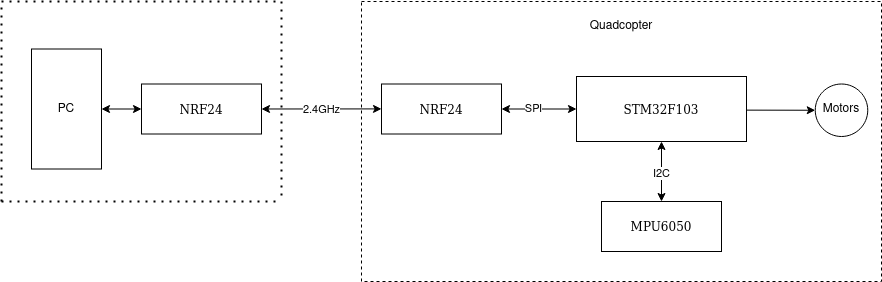
\includegraphics[width=\columnwidth]{img/diagram.png}
\end{center}

\dumblang{Kod do odczytu danych z sensorów oraz regulacji silników jest skonstruowany według następującego schematu blokowego.}\
{The code for reading the sensor data and motor regulation is made according to the block diagram below.}
%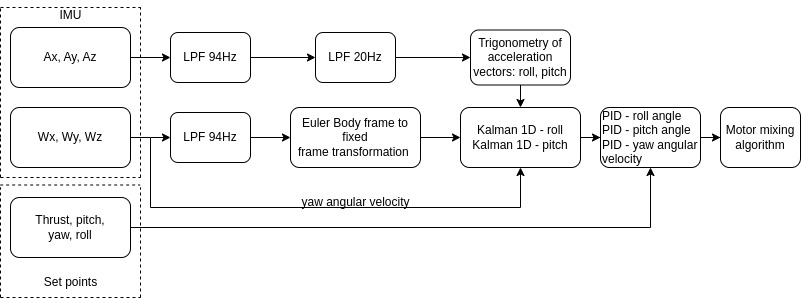
\includegraphics[width=\paperwidth]{img/dsp.jpg}
\begin{center}
 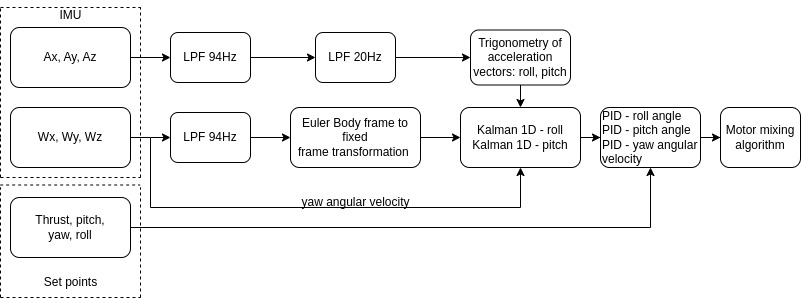
\includegraphics[width=\columnwidth]{img/dsp.jpg}
\end{center}


\section{\dumblang{Opis programu}{Code description}}

\dumblang
% Polish version
{


}
% English version
{
\subsection{nrf24l01 library}
\begin{itemize}
    \item \texttt{HAL\_StatusTypeDef NRF24L01\_Init(NRF24L01\_STRUCT *nrf24l01, \\
    NRF24L01\_CONFIG *nrf24l01\_cfg); }\\
    - Initializes the 2.4Ghz module and sets the default setting
    
    \item \texttt{HAL\_StatusTypeDef NRF24L01\_Enable\_ACKN\_Payload(NRF24L01 \\ *nrf24l01); } \\
    - Enables acknowledge payloads support. Thanks to it, you can immediately send a message to 
    the radio that previously transmitted the data.
    
    \item \texttt{HAL\_StatusTypeDef NRF24L01\_Open\_Reading\_Pipe(NRF24L01\_STRUCT *nrf24l01, uint8\_t pipeAddr, uint64\_t rxAddr, uint8\_t payloadSize);}\\
    - Opens a pipe through which messages from the transmitter will be received.

    \item \texttt{HAL\_StatusTypeDef NRF24L01\_Get\_Info(NRF24L01\_STRUCT *nrf24l01);} \\
    - Reads all nrf24l01 status registers, used for debugging.
    
    \item \texttt{HAL\_StatusTypeDef NRF24L01\_Read\_PayloadDMA(NRF24L01\_STRUCT \\ *nrf24l01, uint8\_t len);} \\
    - Reads the payload sent by the transmitter using SPI in combination with the DMA (direct memory access controller).
    
    \item \texttt{void NRF24L01\_Read\_PayloadDMA\_Complete(NRF24L01\_STRUCT \\ 
    *nrf24l01, uint8\_t *data, uint8\_t len);}\\
    - After receiving data from the radio using DMA, it saves it to the given buffer.
    
    \item \texttt{HAL\_StatusTypeDef NRF24L01\_Write\_ACKN\_Payload(NRF24L01\_STRUCT \\
    *nrf24l01, void *data, uint8\_t len);}\\
    - Saves data that will be sent after receiving the next message from the transmitter.

    \item  \texttt{HAL\_StatusTypeDef NRF24L01\_Start\_Listening(NRF24L01\_STRUCT *nrf24l01);} \\
    - Starts listening for incoming packets and enables interrupts from nrf24l01.

    \item  \texttt{void NRF24L01\_Stop\_Listening(NRF24L01\_STRUCT *nrf24l01)}
    - Stops listening for incoming packets and disables interrupts from nrf24l01.
\end{itemize} 
\subsection{rc library}
\begin{itemize}
    \item \texttt{void RC\_Receive\_Message(uint8\_t message[8], RC\_t *rc)} \\
    - Turns the received message into a control structure that is used to control the quadcopter
\end{itemize}
\subsection{angle\_estimation library}
    \begin{itemize}
    \item \texttt{void Estimate\_Angles\_Init(float dt, float alpha, float tau)}\\
    - Initialize Angle estimator: dt - sampling time, alpha - coefficient for complementary filter, tau - coefficient for accelerometer low\-pass filters, $\tau = \frac{1}{2 \pi f}$.
    \item  \texttt{void Estimate\_Angles(float angles[2], float angular\_velocities[3], \\
    float acc\_buf[3], float gyro\_buff[3])} \\
    - Calculates angles using trigonometry of acceleration vectors and transforms body frame to fixed frame using Euler rotation matrix. Finally, it combines these two readings using Kalman Filters or Complementary filters and thus estimates the angles at which the drone is located.
    \end{itemize}
}
\subsection{stabilizer library}
    \begin{itemize}
        \item \texttt{void Stabilizer\_init()} \\
        - Sets all PIDs and filters needed to stabilize the quadcopter.
        \item \texttt{void Stabilize(float angles[2], float angular\_velocities[3], \\
        int8\_t control\_inputs[4])} \\
        - Stabilizes the drone's movement using PID controllers.
    \end{itemize}

\subsection{motors library}
    \begin{itemize}
        \item \texttt{void Motors\_SetPWR(uint8\_t thrust, int8\_t yaw, int8\_t pitch, int8\_t roll)} \\
        - Using the Motor Mixing Algorithm sets the pwm of all four motors.
        \item  \texttt{void Motors\_Switch(uint8\_t power\_on)} \\
        - Turns the motors on and off.
    \end{itemize}

\subsection{MPU6050 library}
    \begin{itemize}
        \item \texttt{MPU6050\_STRUCT} - a structure tpye containing the I$^2$C address of MPU6050 and addresses of buffers for the data being read.
        \item \texttt{MPU6050\_config} - structure type for MPU configuration
        \item \texttt{MPU6050\_config MPU\_get\_default\_cfg(void)} - returns the default configuration for MPU
        \item \texttt{HAL\_StatusTypeDef MPU\_init(MPU6050\_STRUCT *mpu, MPU6050\_config* cfg)} - initialises the MPU according to the config passed as argument. 
        \item \texttt{HAL\_StatusTypeDef MPU\_measure\_gyro\_offset(MPU6050\_STRUCT* mpu, uint16\_t samples} - measures the constant offset of the gyroscope based on set sample number.
        \item \texttt{HAL\_StatusTypeDef MPU\_measure\_acc\_offset(MPU6050\_STRUCT* mpu, uint16\_t samples)} - measures the constant offset of the accelerometer.
        \item \texttt{HAL\_StatusTypeDef MPU\_clear\_int(MPU6050\_STRUCT *mpu)} - clears the interrup flag from MPU's interrupt status register.
        %\item \texttt{HAL_StatusTypeDef MPU_read_acc(MPU6050_STRUCT *mpu, FLOAT_TYPE output[])} - reads the accelerometer output to the \texttt{output[]}
        %\item \texttt{HAL_StatusTypeDef MPU_read_gyro(MPU6050_STRUCT *mpu, FLOAT_TYPE output[])} - reads the gyroscope output to the \texttt{output[]}
        \item \texttt{HAL\_StatusTypeDef MPU\_read\_acc\_gyro\_DMA(MPU6050\_STRUCT *mpu)} - reads accelerometer and gyroscope data using DMA to a memory location passed using the config struct.
        \item \texttt{HAL\_StatusTypeDef MPU\_read\_acc\_gyro\_DMA\_complete(MPU6050\_STRUCT *mpu)} - calculates the sensor values from raw bytes after the readout has been completed.
    \end{itemize}

    Note that the functions for measuring the offsets write the result to a static variable defined in the library source file. The functions for reading the measurements of the IMU substract the offsets automatically.
%\section{Schemat elektryczny}

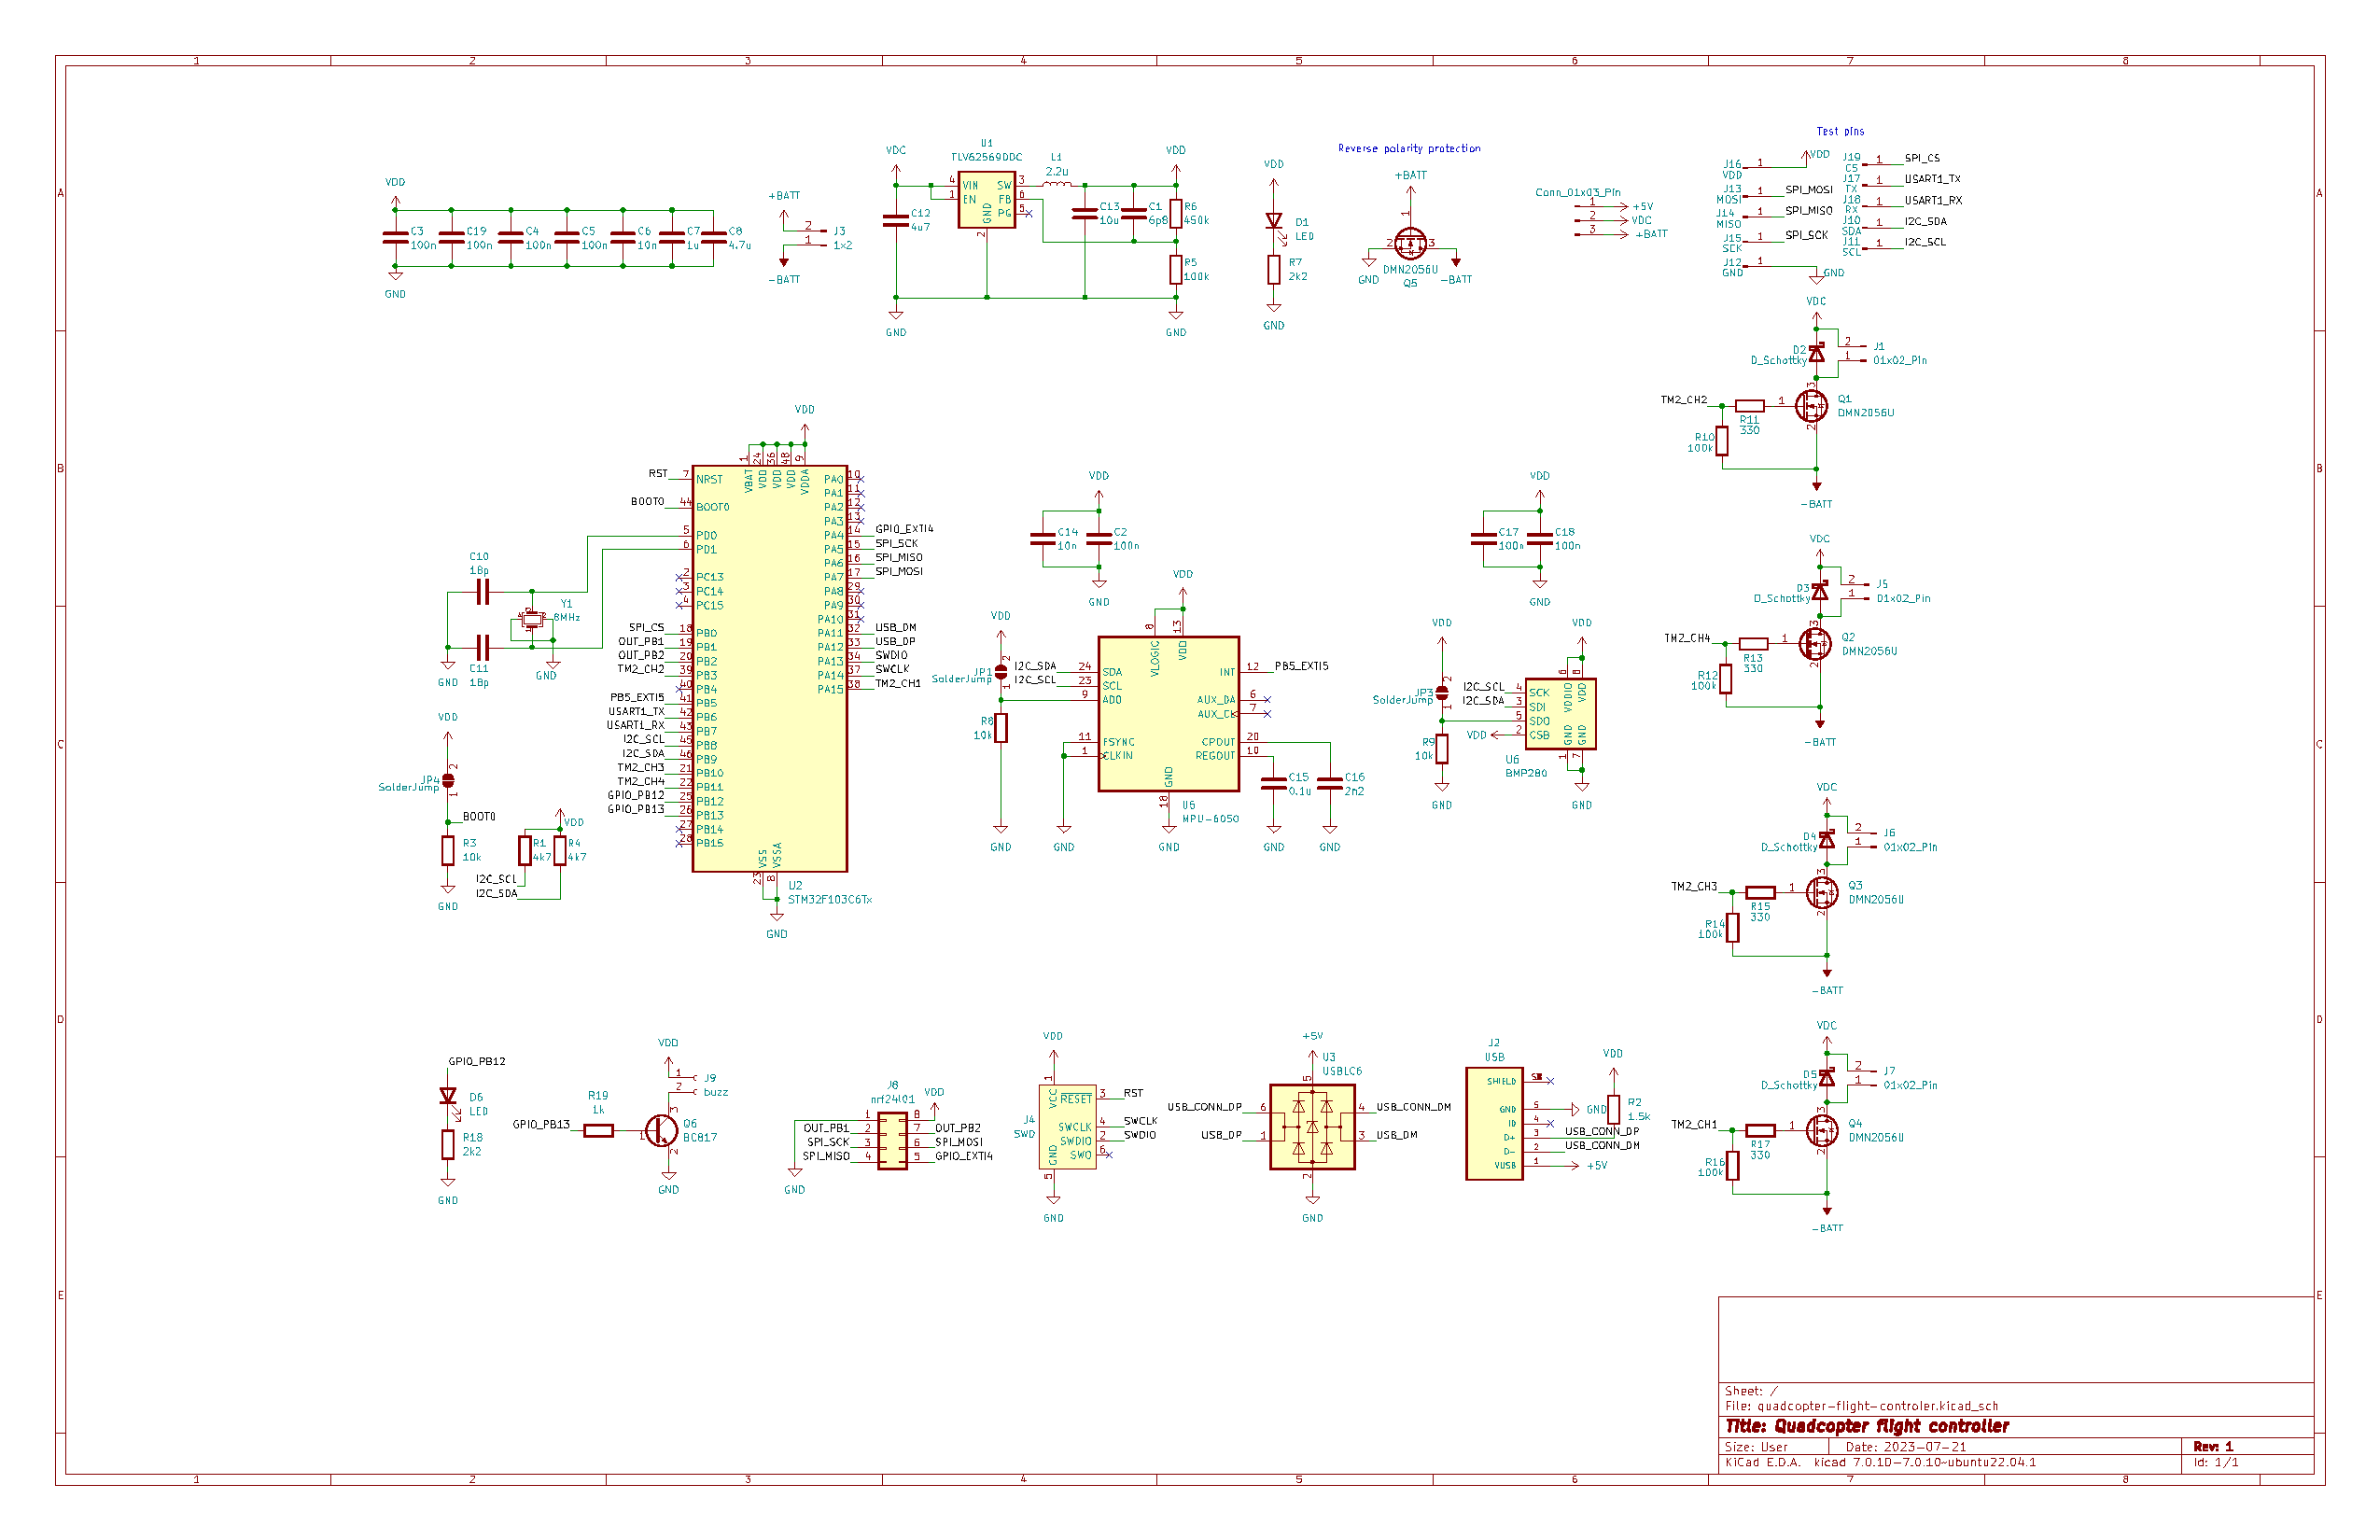
\includepdf[fitpaper=true, pages=-]{dron_schemat.pdf}

\begin{center}
 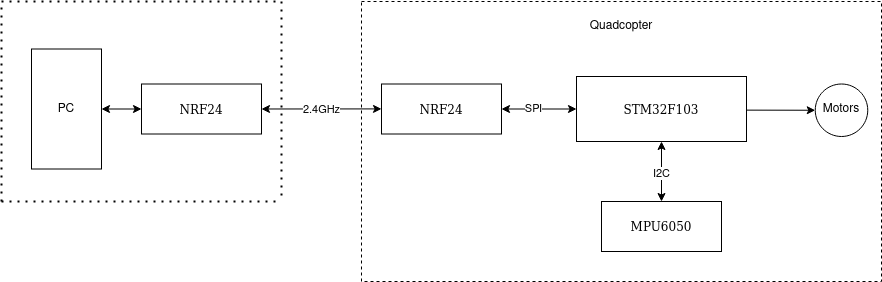
\includegraphics[width=\columnwidth]{img/diagram.png}
\end{center}

\include

\end{document}
